\subsectionold{x86}

\subsubsectionold{MSVC}

Компилируем:

\lstinputlisting[caption=MSVC 2008]{patterns/13_arrays/1_simple/simple_msvc.asm}

\myindex{x86!\Instructions!SHL}
Ничего особенного, просто два цикла. Один изменяет массив, второй печатает его содержимое. 
Команда \INS{shl ecx, 1} используется для умножения \ECX на 2, об этом ниже~(\myref{SHR}).

Под массив выделено в стеке 80 байт, это 20 элементов по 4 байта.

\clearpage
Попробуем этот пример в \olly.
\myindex{\olly}

Видно, как заполнился массив: каждый элемент это 32-битное слово типа \Tint, с шагом 2:

\begin{figure}[H]
\centering
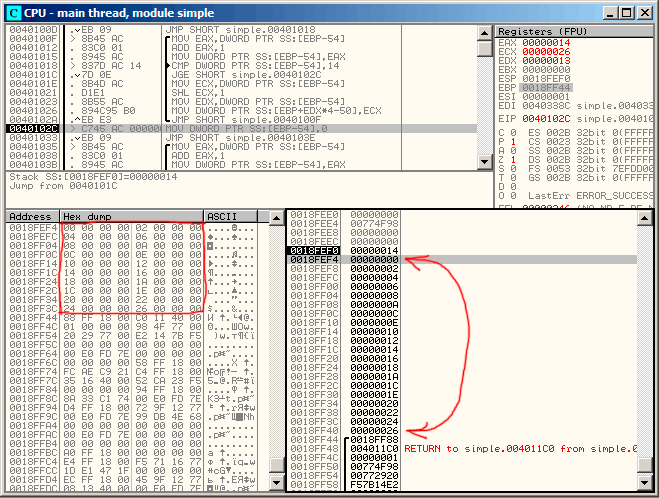
\includegraphics[scale=\FigScale]{patterns/13_arrays/1_simple/olly.png}
\caption{\olly: после заполнения массива}
\label{fig:array_simple_olly}
\end{figure}

А так как этот массив находится в стеке, то мы видим все его 20 элементов внутри стека.

\subsubsectionold{GCC}

Рассмотрим результат работы GCC 4.4.1:

\lstinputlisting[caption=GCC 4.4.1]{patterns/13_arrays/1_simple/simple_gcc.asm}

Переменная $a$ в нашем примере имеет тип \IT{int*} (указатель на \Tint{}).
Вы можете попробовать передать в другую функцию указатель на массив,
но точнее было бы сказать, что передается указатель на первый элемент массива
(а адреса остальных элементов массива можно вычислить очевидным образом).

Если индексировать этот указатель как \IT{a[idx]}, \IT{idx} просто прибавляется к указателю 
и возвращается элемент, расположенный там, куда ссылается вычисленный указатель.

Вот любопытный пример. Строка символов вроде \IT{\q{string}} это массив из символов. 
Она имеет тип \IT{const char[]}.
К этому указателю также можно применять индекс.

Поэтому можно написать даже так:  \TT{\q{string}[i]}~--- это совершенно легальное выражение в \CCpp!

